\documentclass{article}

% if you need to pass options to natbib, use, e.g.:
%     \PassOptionsToPackage{numbers, compress}{natbib}
% before loading neurips_2018

% ready for submission
% \usepackage{neurips_2018}

% to compile a preprint version, e.g., for submission to arXiv, add add the
% [preprint] option:
%     \usepackage[preprint]{neurips_2018}

% to compile a camera-ready version, add the [final] option, e.g.:
\usepackage[final]{neurips_2018}

% to avoid loading the natbib package, add option nonatbib:
%     \usepackage[nonatbib]{neurips_2018}

\usepackage[utf8]{inputenc} % allow utf-8 input
\usepackage[T1]{fontenc}    % use 8-bit T1 fonts
\usepackage{hyperref}       % hyperlinks
\usepackage{url}            % simple URL typesetting
\usepackage{booktabs}       % professional-quality tables
\usepackage{amsfonts}       % blackboard math symbols
\usepackage{nicefrac}       % compact symbols for 1/2, etc.
\usepackage{microtype}      % microtypography


\usepackage{srcltx,pdfsync}
%\usepackage[pdflatex=false,recompilepics]{gastex} subfigure
\usepackage{amsmath,amssymb}
\usepackage{geometry}
\usepackage{graphicx,wrapfig}
\usepackage{subcaption}

\usepackage{pdflscape}

\usepackage{ifthen}

\def\Lap{\ensuremath{\mathcal{L}}}

\graphicspath{{./Images/}}

\title{GAN and VAE for MNIST}

% The \author macro works with any number of authors. There are two commands
% used to separate the names and addresses of multiple authors: \And and \AND.
%
% Using \And between authors leaves it to LaTeX to determine where to break the
% lines. Using \AND forces a line break at that point. So, if LaTeX puts 3 of 4
% authors names on the first line, and the last on the second line, try using
% \AND instead of \And before the third author name.

\author{%
	Ninad K.~Gaikwad
	Department of Mechanical and Aerospace Engineering\\
	University of Florida\\
	Gainesville, FL 32611 \\
	\texttt{ninadgaikwad@ufl.edu} \\
}

\begin{document}
	% \nipsfinalcopy is no longer used
	
	\maketitle
	
	\begin{abstract}
	
	In this paper Generative Adversarial Networks (GAN) and Variational Autoencoders (VAE) have been used to learn images of handwritten digits. Three models of GANs and two models of VAEs have been trained on the data-set so as to generate new images which look like hand written digits. It is observed that VAE models perform better than their GAN counterparts. However, training both types of models involves optimized selection of numerous hyper-parameters which makes them hard to train. Code for the paper can be accessed at \url{https://github.com/ninadkgaikwad/CAP6610}
	
	\end{abstract}
	
	\section{Introduction}\label{section:Introduction}
	
	The goal of generative modeling is to learn the underlying probability distribution of the data. Once we have that distribution; firstly we have completely characterized the data and secondly we can sample from the distribution to generate new data which has all the characteristics of the other data belonging to the distribution. So, if we are able to learn the underlying probability distribution of handwritten digits images we can generate completely new images which we exactly look like handwritten digits. This generative power of these models is useful now than ever before as they can be used to to generate data for supervised learning algorithms, time series data required by Reinforcement learning algorithms can be generated, and finally useful general features of a dataset can be extracted by inferring latent variables.
	
	The rest of this paper is organized as follows. Section~\ref{section:GanAndVae} describes the fundamentals of GAN and VAE. Section~\ref{section:ExperimentSetup} presents the GAN and VAE model development and hyper-parameter section. Results obtained from trained GANs and VAEs are presented and discussed in Section~\ref{section:ResultsDiscussion}.  Finally, the main conclusions are provided in Section~\ref{section:Conclusion}.	
		
	\section{GAN and VAE basics}\label{section:GanAndVae}
	
	
	\subsection{Generative Adverserial Networks}\label{subsection:Gan}
	
	GAN was introduced in \cite{GoodfellowGenerative:2014} as a model to implicitly learn the probability distribution of the data ($P_{data}$) implicitly so that new data of the same characteristics can be sampled from it. 
	
	It has two parts the generator ($G(z;\theta_{g})$)) and the discriminator ($D(x;\theta_{d})$)), where $z\sim P_{z}=\mathcal{N}(0,1)$  is noise prior which can be used to sample from the ($G(z;\theta_{g})$)), and $x\sim P_{data}$ is the data.
	
	Now, we want $G(z;\theta_{g}) = P_{data}$ so that when we sample from generator we get data similar to that from $P_{data}$. In order for the generator to learn the data distribution GAN proposes an adversary in the form of the discriminator which tries to find the probability of the data sample coming from the data distribution, hence $D(x;\theta_{d})=P_{data}(x)/(P_{data}(x)+P_{g}(x))$. 
	
	Now, the discriminator can give low probability to data coming from the generator if the generator is not good enough. Therefore, to train the generator to achieve its goal it plays a two-player minmax game with the discriminator as follows;
	
	\begin{align} 
		\min_{G} \max_{D} V(D,G) &= \mathcal{E}_x\sim P_{data}(logD(x)) + {E}_z\sim P_{z}(1-logD(G(z))). \nonumber
	\end{align} 

	Hence the above loss is maximized over the $D(x;\theta_{d})$ while ${E}_z~P_{z}(1-logD(G(z)))$ is minimized over the $G(x;\theta_{g})$. Both the above losses can be computed as cross-entropy losses, where both $G(z;\theta_{g}) = P_{data}$ and $D(x;\theta_{d})=P_{data}(x)/(P_{data}(x)+P_{g}(x))$ are be neural networks, as the generator and discriminator represent complex probability distributions.     
	
	\subsection{Variational Autoencoders}\label{subsection:Vae}
	
	Variational Autoencoders were introduced in \cite{kingmaIntroduction:2019} as a model to learn the conditional probability distributions between data ($x$) and its latent variable ($z$) where;  $z \sim P_{\theta}(z)= \mathcal{N}(\mu,\Sigma)$. Now if we want to generate data from the latent variable we need $P_{\theta}(x|z)$, this is a complex probability distribution and can be represented by a neural network, this neural network is the decoder in VAE.
	
	Now, from standard probability theory we know $P_{\theta}(x)= \int P_{\theta}(z)P_{\theta}(x|z)dz$ and $P_{\theta}(z|x)=P_{\theta}(x|z)P_{\theta}(z)/P_{\theta}(x)$, we should note that we don't know $P_{\theta}(x)$ and we want to learn $P_{\theta}(x|z)$, hence the integral is intractable and we cannot use the standard maximum likelihood estimation technique. 
	
	To over come this problem VAE comes up with its encoder which approximatethe conditional probability distribution $P_{\theta}(z|x)$ as $q_{\phi}(z|x)$. Now we can find a lower bound for the log-likelihood of $P_{\theta}(x)$ as follows;
	
	\begin{align} 
	\log P_{\theta}(x^{(i)}) &= E_{z \sim q_{\phi}(z|x)}  \left[ \log P_{\theta}(x)  \right] \quad \text{\emph{($P_{\theta}(x)$ does not depend on $z$)}} \nonumber \\
	&= E_{z \sim q_{\phi}(z|x)}  \left[ \log \dfrac{P_{\theta}(x|z)P_{\theta}(z)}{P_{\theta}(z|x)}  \right] \quad \text{\emph{(Baye's Rule)}} \nonumber \\
	&= E_{z \sim q_{\phi}(z|x)}  \left[ \log \dfrac{P_{\theta}(x|z)P_{\theta}(z)}{P_{\theta}(z|x)} \dfrac{q_{\phi}(z|x)}{q_{\phi}(z|x)} \right] \quad \text{\emph{(Multiplying and dividing by $q_{\phi}(z|x)$ )}} \nonumber \\
	&= E_{z \sim q_{\phi}}  \left[ \log P_{\theta}(x|z) \right] - E_{z \sim q_{\phi}}  \left[ log \dfrac{q_{\phi}(z|x)}{P_{\theta}(z)}\right] +E_{z \sim q_{\phi}}  \left[ log \dfrac{q_{\phi}(z|x)}{P_{\theta}(z|x)} \right] \label{eq:VAE2} \\
	&= E_{z \sim q_{\phi}}  \left[ \log P_{\theta}(x|z) \right] - D_{KL}\left( q_{\phi}(z|x) || P_{\theta}(z) \right) + D_{KL}\left( q_{\phi}(z|x) || P_{\theta}(z|x) \right). \label{eq:VAE1}
	\end{align} 	
	
	Now, from (eq.~(\ref{eq:VAE1})) the first part is tractable as decoder provides $P_{\theta}(x|z)$, the second part is tractable as $q_{\phi}(z|x) $ and $P_{\theta}(z|x)$ can be assumed to be of normal distribution as the prior $P_{\theta}(z)= \mathcal{N}(\mu,\Sigma)$ and then we have a closed form solution for their KL divergence, but third part is not tractable but as it is too a KL divergence will always be non-negative, hence we find the lower bound on $\log P_{\theta}(x^{(i)})$ as $ \log P_{\theta}(x^{(i)}) \geq E_{z \sim q_{\phi}}  [ \log P_{\theta}(x|z) ] - D_{KL}( q_{\phi}(z|x) || P_{\theta}(z) ) $ this is called the Variational Lower Bound (VLB), and now we can maximize the lower bound to in turn maximize the $\log P_{\theta}(x^{(i)})$. Now from (eq.~(\ref{eq:VAE2})) by using Elbow Loss can also be written as;
	
	\begin{align} 
	VLB = E_{z \sim q_{\phi}}  \left[ \log P_{\theta}(x|z) \right] - E_{z \sim q_{\phi}}  \left[ log q_{\phi}(z|x)\right] + E_{z \sim q_{\phi}}\left[\log P_{\theta}(z)\right]. \label{eq:VAE3}
	\end{align} 
	
	Now, from (eq.~(\ref{eq:VAE3})) we see that; the first part can be computed using cross-entropy loss, whereas the second and third part are the log-likelihoods of respective normal distributions, hence we can compute these using the following for a $w \sim \mathcal{N}(\mu_w,\sigma^{2}_{w})$	as follows;
	
	\begin{align} 
	\log P(w) &= -\log (\sigma_{w}) - \dfrac{1}{2}\log (2\pi) - \dfrac{(w-\mu_{w})^2}{2\sigma^{2}} , \label{eq:VAE4}
	\end{align}
	
	As, we can now compute our Variational Lower Bound or the loss we can perform gradient descent and update the parameters $\theta$ and $\phi$. However, as there is sampling operation of $z \sim \mathcal{N}(\mu,\Sigma)$, we cannot compute gradients directly. We need to parameterize $z=g(\mu_{x|z},\Sigma_{x|z},\epsilon)$ where $\mu_{x|z},\Sigma_{x|z}$ are obtained from the encoder and $\epsilon \sim {N}(0,1)$ is the auxiliary noise variable, this called the reparameterization trick. One particular example of $g(\mu_{x|z},\Sigma_{x|z},\epsilon)$ is $z = \mu_{z|x} + \epsilon \sigma_{z|x} $.	

	\section{Experiment Setup}\label{section:ExperimentSetup}
	This section describes the experiment setup in detail.
	
	\subsection{Software and Hardware}\label{subsection:SoftwareHardware}
	

	\paragraph{Software} Programming language used is \emph{Python 3.6}, and the integrated development environment is \emph{Spyder}. The \emph{tensorflow} package has been used for data processing, creating and training the models.

	\paragraph{Hardware} 64bit 16GB 8$\times$1.80GHz Windows 10 Machine without a CUD enabled GPU was used for training the models.	
	
	\subsection{Data Preprocessing}\label{subsection:DataPreprocessing}
	
	The MINST dataset is used to develop generative models which can produce images of handwritten digits. It consists of $60000$ training and 10000 testing examples of handwritten images along with labels. These images are grey-scale with a size of $28\times28$, with each element in the image between $[0,255] \in \mathbb{Z}$. For performing an effective and converging gradient descent during learning the training image elements need to be scaled down either to $[-1,1] \in \mathbb{R}$ or $[0,1] \in \mathbb{R}$, which can be done as follows;
	
	\begin{align}
	x_{processed} &= \dfrac{x_{original} - 127.5}{127.5}, \label{eq:Data1} \\
	x_{processed} &= \dfrac{x_{original}}{255}, \label{eq:Data2} 
	\end{align}
	
	where, (eq.~(\ref{eq:Data1})) scales the image elements between $[-1,1]$, and  (eq.~(\ref{eq:Data2})) scales them between $[0,1]$. These images are further shuffled and grouped together as batches of equal number of images per batch (Batch Size). Each of these batches is used to compute the loss function during one gradient update step. When gradients have been updated sequentially iterating through all the batches this is called as one Epoch. The gradients are updated for multiple epochs till the model is sufficiently trained. 	   
	
	
	\subsection{GAN and VAE Architectures}\label{subsection:GanVaeArchitecture}
	
	Table~\ref{table:GANArchitecture} shows the layers of the three GANs developed: DenseGAN which consists of only fully connected layers and no convolutional neural nets (CNN) are used, DenseGAN-Deep is also consists fully connected layers, and CNNGAN consists of majority of CNNs and some fully connected layers near the input and output layers. 
	
	
	\begin{table}[t]
		\caption{Network architectures for GAN}
		\label{table:GANArchitecture}
		\centering
		\begin{tabular}{lclclcl}
			
			\toprule
			
			Network Type & Generator Network Layers & Discriminator Network Layers \\
			
			\midrule
			
			DenseGAN-Deep-1   & Input(392)     	        & Input(28,28)  \\
			DenseGAN-Deep-2   & Dense(100)    	        & Reshape(784)  \\
			DenseGAN-Deep-3   & Dense(200)     	        & Dense(600)  \\
			DenseGAN-Deep-4   & Dense(300)     	        & Dense(500)  \\
			DenseGAN-Deep-5   & Dense(400)     	        & Dense(400)  \\
			DenseGAN-Deep-6   & Dense(500)     	        & Dense(300)  \\
			DenseGAN-Deep-7   & Dense(600)     	        & Dense(200)  \\
			DenseGAN-Deep-8   & Dense(784)     	        & Dense(100)  \\
			DenseGAN-Deep-9   & Reshape(28,28)     	    & Dense(1)  \\
			
			\midrule
			
			DenseGAN-1   & Input(10)     	     & Input(28,28)  \\
			DenseGAN-2   & Dense(100)     	     & Reshape(784)  \\
			DenseGAN-3   & Dense(300)     	     & Dense(600)  \\		
			DenseGAN-4   & Dense(600)     	     & Dense(300)  \\		
			DenseGAN-5   & Dense(784)     	     & Dense(100)  \\
			DenseGAN-6   & Reshape(28,28)     	 & Dense(1)  \\
			
			\midrule
			
			CNNGAN-1   & Input(10)     	        		& Input(28,28)  \\
			CNNGAN-2   & Dense(7*7*128)     	        & Conv2D(32,5,2)  \\
			CNNGAN-3   & Reshape(7,7,128)     	        & Conv2D(64,5,2)  \\		
			CNNGAN-4   & Conv2DTranspose(64,5,2)     	& Conv2D(128,5,2)  \\		
			CNNGAN-5   & Conv2DTranspose(32,5,1)     	& Flatten()  \\
			CNNGAN-6   & Conv2DTranspose(1,5,2)     	& Dense(1)  \\		
			
			\bottomrule
		\end{tabular}
	\end{table}

	Table~\ref{table:VAEArchitecture} shows the layers of the two VAEs developed: DenseVAE which consists of only fully connected layers and no convolutional neural nets (CNN) are used, and VAEGAN consists of majority of CNNs and some fully connected layers near the input and output layers. 

	\begin{table}[t]
		\caption{Network architectures for VAE}
		\label{table:VAEArchitecture}
		\centering
		\begin{tabular}{lclclcl}
			
			\toprule
			
			Network Type & Decoder Network Layers & Encoder Network Layers \\
			
			\midrule
			
			DenseVAE-1   & Input(4)     	        & Input(28,28)  \\
			DenseVAE-2   & Dense(50)    	        & Reshape(784)  \\
			DenseVAE-3   & Dense(100)     	        & Dense(600)  \\
			DenseVAE-4   & Dense(300)     	        & Dense(300)  \\
			DenseVAE-5   & Dense(600)     	        & Dense(100)  \\
			DenseVAE-6   & Dense(784)     	        & Dense(50)  \\
			DenseVAE-7   & Reshape(28,28)     	    & Dense(4)  \\
			
			\midrule
			
			CNNVAE-1   & Input(10)     	        		& Input(28,28)  \\
			CNNVAE-2   & Dense(7*7*128)     	        & Conv2D(32,5,2)  \\
			CNNVAE-3   & Reshape(7,7,128)     	        & Conv2D(64,5,2)  \\		
			CNNVAE-4   & Conv2DTranspose(64,5,2)     	& Conv2D(128,5,2)  \\		
			CNNVAE-5   & Conv2DTranspose(32,5,1)     	& Flatten()  \\
			CNNVAE-6   & Conv2DTranspose(16,5,2)     	& Dense(1)  \\
			CNNVAE-6   & Conv2DTranspose(1,5,2)     	&   \\		
			
			\bottomrule
		\end{tabular}
	\end{table}	

	In both GAN and VAE model layer descriptions in Table~\ref{table:GANArchitecture} and Table~\ref{table:VAEArchitecture} all the layers except the Input() and Reshape() layers are followed by Batch-Normalization layers as it helps with standardizing the inputs to every layer. This stabilizes the learning process in deep neural networks and helps in reducing the number of epochs required to train. ReLu activation function is used after every Batch Normalization layer, it helps with the vanishing gradient problem caused classical activation functions like Sigmoid and TanH.
	
	Symmetry of generator-discriminator in GAN and encoder-decoder in VAE is maintained in the architecture.  
	
	\subsection{Hyperparameter Selection}\label{subsection:Hyperparameter}
	
	Table~\ref{table:Hyperparameter} presents the hyper-parameters selected for both GAN and VAE models. \cite{GoodfellowNips:2016,} and \cite{kingmaIntroduction:2019} were helpful in the designing and training of the GAN and VAE models repectively.
				
	\begin{table}[t]
		\caption{Network architectures for VAE}
		\label{table:Hyperparameter}
		\centering
		\begin{tabular}{lclclcl}
			
			\toprule
			
			Hyperparameter Type & GAN & VAE \\
			
			\midrule
			
		    GAN Noise Dimesion    			&	392 and 10,     & N.A  \\
											&       	        &    \\
			VAE Latent Variable Dimension   & N.A     	    & 10    \\
											&      	        &   \\
											
			\midrule
														
			Total Epochs 					& 50     	    & 50   \\
						  					&      	        &   \\
		    Batch Size    					& 128     	    & 128  \\
		    			  					&      	        &   \\
		    			  					
		    \midrule
		    			  					
		    Optimizer    					& ADAM     	    & ADAM   \\
						 					&      	        &   \\
		    Learning Rate				    &$10^{-5}$,$10^{-6}$,$10^{-4}$ & $10^{-4}$    \\
		    		        
											&      	        &   \\
											
			\midrule
								  	
		    Activation for Layers    		& ReLu      	& ReLu   \\
											&      	        &   \\
		    Batch Normalization for Layers  & ReLu 			& ReLu   \\
											&      	        &   \\
											
			\midrule

		    Filter Size for CNNs    		& 16, 32, 64, 128     	& 16, 32, 64, 128  \\
											&      	        		&   \\
											
		    Kernel Size for CNNs    		& (5,5)     	& (5,5)  \\
											&      	        &   \\
		    Padding for CNNs    			& 'same'     	& 'same'   \\
											&      	        &   \\
		    Stride for CNNs    				&(1,1) and (2,2)&(1,1) and (2,2)   \\
											&      	        &   \\
	
		    Output size of CNNs    			&(7,7),(14,14),(28,28)& (7,7), (14,14), (28,28)   \\
											&      	        &   \\
		
			\bottomrule
		\end{tabular}
	\end{table}

	The GAN noise dimension used in DenseGAN is 392 = 28*28/2, was selected to see if a fully connected layer GAN can perform good with half the output datasize, while the npoise dimension of 10 used for the other two GAN models is fairly standard for MNIST dataset. The latent variable dimension of 2 used for the other two VAE models is fairly standard for MNIST data. 

	Batch sizes are usually multiples 16 and some common ones are: 16, 32, 128, 256; smaller batch sizes takes us closer to stochastic gradient descent (SGD) which helps in updating networks wieghts frequently as compared traditional gradient descent (GD) which needs to compute the gradients over all the training examples, hence a batch size of 128 was selected. However, gradients of SGD are noisy, hence to combine the best of SGD and GD mini-batch stochastic gradient is used. There are various other optimizers which create a better wieght update than SGD with mini-batches like Adam, adagrad, and Nadam, they do this by reducing the noise in wieght updates using momentum terms and adapative learning rates, hence ADAM was chosen. Learning rates were selected for each problem by looking at the Loss vs. Epoch curves. 
	
	For CNN layers filter sizes can be any positive integer, however kernel sizes of powers of two are commonly used for images, in the GAN and VAE architectures presented in this paper filter sizes increase from 16 to 128 in the generator and decoder whereas.Kernel sizes can be anything, usually for images (3,3), (5,5) and (7,7) are used, hence as middle ground (5,5) was chosen for all CNNs in both GAN and VAE models. Padding was selected to 'same'- creates padding such that with stride(1,1) the size of input and output of the CNN layer is same. Strides are the jumps the CNN makes while moving over the 2D image surface, when padding is selected as 'same' down-sampling by half can be achieved using stride of (2,2) in Conv2D() layer and up-sampling by factor of two can be achieved using stride of (2,2) in Conv2DTranspose() layer. Hence, as the training image size is (28,28) it can be down-sampled to (14,14) and (7,7) in GAN discriminator, and VAE encode; while it can be up-sampled from any noise or latent dimension to (7,7) then upsampled in stages to (28,28) in GAN generator, and VAE decoder.
	
	\cite{TensorFlowCNNVAE:online} and \cite{TensorflowCNNVAE:online} were very helpful resources for understanding the programming aspects GANs and VAEs in python using TesorFlow.
	
	
	\section{Results and Discussion}\label{section:ResultsDiscussion}
	
	This section illustrates and discusses about the results obtained from the trained GAN and VAE models.
	
	\begin{figure*}[htbp]
		\centering
		\begin{subfigure}[t]{0.32\textwidth}
			\centering
			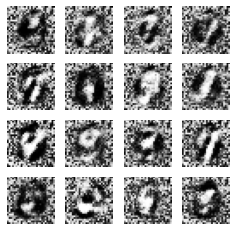
\includegraphics[scale=0.39]{GAN_Dense_GenImage.png}
			\caption{DenseGAN.}
			\label{fig:GANImage_1}
		\end{subfigure}
		\begin{subfigure}[t]{0.32\textwidth}
			\centering
			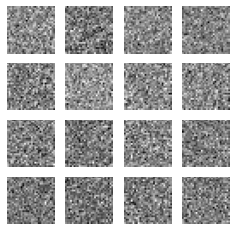
\includegraphics[scale=0.39]{GAN_Dense_GenImage_Deep.png}
			\caption{DenseGAN-Deep.}
			\label{fig:GANImage_2}
		\end{subfigure}
		\begin{subfigure}[t]{0.32\textwidth}
			\centering
			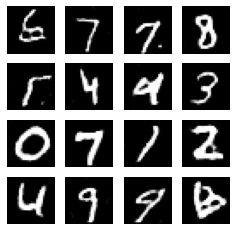
\includegraphics[scale=0.39]{GAN_CNN_GenImage.png}
			\caption{CNNGAN.}
			\label{fig:GANImage_3}
		\end{subfigure}
		\caption{ Images generated by the three different GAN architectures: DenseGAN, DenseGAN-Deep, and CNNGAN.}
		\label{fig:ResultsGANImages}
	\end{figure*}

	Figure~\ref{fig:ResultsGANImages} shows output of the generator of  DenseGAN, DenseGAN-Deep and CNNGAN from left to right respectively, it can be easily seen that CNNGAN's output resembles handwritten digits to an extent; however, DenseGAN and DenseGAN-Deep have failed to generate any kind of meaningful handwritten digits. But, in comparison DenseGAN's output seems to find some pattern in the middle of the images which shows on the surface that. This shows that fully connected layer GAN networks work poorly as compared to CNN based GAN networks.
	
	\begin{figure*}[htbp]
		\centering
		\begin{subfigure}[t]{0.32\textwidth}
			\centering
			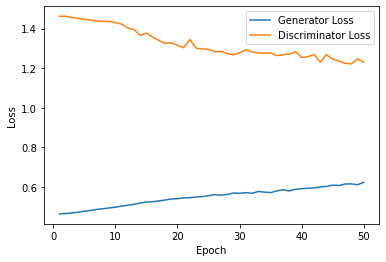
\includegraphics[scale=0.33]{GAN_Dense_LossEpoch.png}
			\caption{DenseGAN.}
			\label{fig:GANLoss_1}
		\end{subfigure}
		\begin{subfigure}[t]{0.32\textwidth}
			\centering
			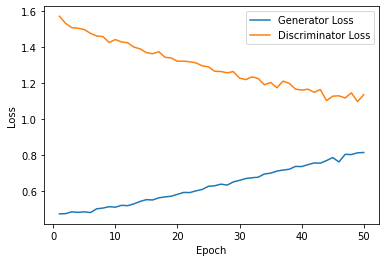
\includegraphics[scale=0.33]{GAN_Dense_LossEpoch_Deep.png}
			\caption{DenseGAN-Deep.}
			\label{fig:GANLoss_2}
		\end{subfigure}
		\begin{subfigure}[t]{0.32\textwidth}
			\centering
			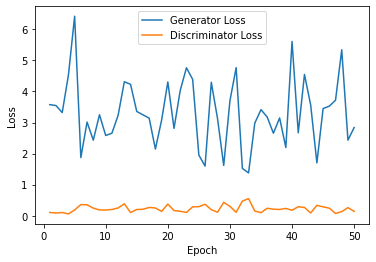
\includegraphics[scale=0.33]{GAN_CNN_LossEpoch.png}
			\caption{CNNGAN.}
			\label{fig:GANLoss_3}
		\end{subfigure}
		\caption{ Generator and Discriminator Loss for all three GAN architectures: DenseGAN, DenseGAN-Deep, and CNNGAN.}
		\label{fig:ResultsGANLoss}
	\end{figure*}

		Figure~\ref{fig:ResultsGANLoss} shows Loss vs. Epoch plots for DenseGAN, DenseGAN-Deep and CNNGAN from left to right respectively. It can be seen that the Dense GANS show a good declining generator loss and increasing generator loss, but this picture does not translate to their learning. While, the Loss vs. Epoch plot of CNNGAN is noisy showing high learning rate the results are beeter than Dense GANs. CNNGAN can perform better with an optimal learning rate.
	
	\begin{figure*}[htbp]
		\centering
		\begin{subfigure}[t]{0.48\textwidth}
			\centering
			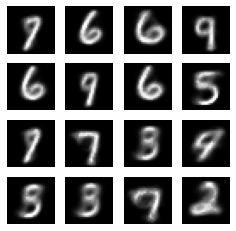
\includegraphics[scale=0.45]{VAE_Dense_GenImage.png}
			\caption{DenseVAE - Generated image.}
			\label{fig:VAEImage_1}
		\end{subfigure}
		\begin{subfigure}[t]{0.48\textwidth}
			\centering
			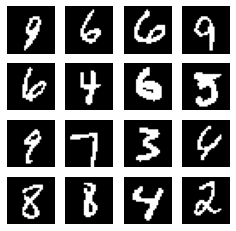
\includegraphics[scale=0.45]{VAE_Dense_RealImage.png}
			\caption{DenseVAE - Real image.}
			\label{fig:VAERealImage_1}
		\end{subfigure}
	
		\begin{subfigure}[t]{0.48\textwidth}
			\centering
			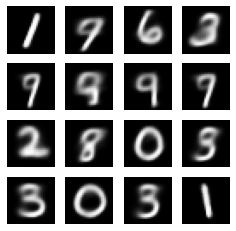
\includegraphics[scale=0.45]{VAE_CNN_GenImage.png}
			\caption{CNNGAN - Generated image.}
			\label{fig:VAEImage_2}
		\end{subfigure}
		\begin{subfigure}[t]{0.48\textwidth}
		\centering
		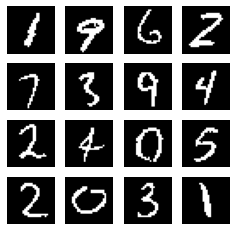
\includegraphics[scale=0.45]{VAE_CNN_RealImage.png}
		\caption{CNNGAN - Real image.}
		\label{fig:VAERealImage_2}
		\end{subfigure}
		\caption{ Images generated by two different VAE architectures: DenseVAE,and CNNVAE against the real respective images.}
		\label{fig:ResultsVAEImages}
	\end{figure*}

	Figure~\ref{fig:ResultsVAEImages} shows output of the decoder of  DenseVAE, and CNNVAE on the left from top to bottom, and real images input to the encoder on the right from top to bottom. We can notice that the outputs of both the VAEs are better than their GAN counterparts in terms of quality, on the other hand the haziness and sharpness of the output images from VAEs and GANS respectively should be noted. We can see that a fully connected network in a VAE framework can work as good as a CNN. However, if you look closely both VAEs are not perfectly trained as there is confusion between 2's and 3's, 4's and 9's etc. The poor training can be seen through Figure~\ref{fig:ResultsVAELoss} which shows the ELBO Loss vs. Epoch plot for DenseVAE and CNNVAE from left to right. It is observed that the learning rate for DENSEVAE is good while for CNNVAE is high, the noise can be attributed to small batch size. These networks can be trained better by optimizing the learning rate and increasing batch size. 
	
	\begin{figure*}[htbp]
		\centering
		\begin{subfigure}[t]{0.48\textwidth}
			\centering
			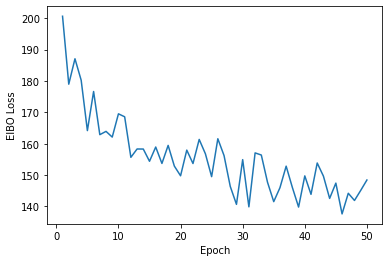
\includegraphics[scale=0.45]{VAE_Dense_LossEpoch.png}
			\caption{DenseVAE.}
			\label{fig:VAELoss_1}
		\end{subfigure}
		\begin{subfigure}[t]{0.48\textwidth}
			\centering
			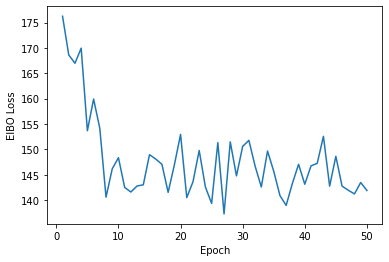
\includegraphics[scale=0.45]{VAE_CNN_LossEpoch.png}
			\caption{CNNVAE.}
			\label{fig:VAERealLoss_1}
		\end{subfigure}
		\caption{ Images generated by two different VAE architectures: DenseVAE,and CNNVAE against the real respective images.}
		\label{fig:ResultsVAELoss}
	\end{figure*}
	
	\section{Conclusion}\label{section:Conclusion}
	Three GAN and two VAE models were trained on the MNIST handwritten digits image dataset. It was seen that these particular architectures of the VAEs performed better than their GAN counterparts, however the VAE output images are hazier while the GAN output images are sharper in comparison. Within the GAN models the fully connected layer models failed to train meaningfully while the CNN layer model trained better. It was also seen that the VAE with just fully connected layers outperformed GAN with CNN in terms of readability of the digits. Overall the VAE models constructed here performed better over the GAN models in terms of readability, but they still were confused on many numbers.
	
	\newpage
	
	\section{References}\label{section:References}
		
	\bibliographystyle{IEEEtran}
	\bibliography{{./BiBFolder/BibFile}}		
	
	
	
\end{document}


\begin{table}
	\caption{Network architectures for GAN}
	\label{table:GANArchitecture}
	\centering
	\begin{tabular}{lclclcl}
		
		\toprule
		
		Network Type & Generator Network Layers & Discriminator Network Layers \\
		
		\midrule
		
		DenseGAN-Deep-1   & Input(392)     	        & Input(28,28)  \\
		DenseGAN-Deep-2   & Dense(100)    	        & Reshape(784)  \\
		DenseGAN-Deep-3   & Dense(200)     	        & Dense(600)  \\
		DenseGAN-Deep-4   & Dense(300)     	        & Dense(500)  \\
		DenseGAN-Deep-5   & Dense(400)     	        & Dense(400)  \\
		DenseGAN-Deep-6   & Dense(500)     	        & Dense(300)  \\
		DenseGAN-Deep-7   & Dense(600)     	        & Dense(200)  \\
		DenseGAN-Deep-8   & Dense(784)     	        & Dense(100)  \\
		DenseGAN-Deep-9   & Reshape(28,28)     	    & Dense(1)  \\
		
		\midrule
		
		DenseGAN-Shallow-1   & Input(10)     	     & Input(28,28)  \\
		DenseGAN-Shallow-2   & Dense(100)     	     & Reshape(784)  \\
		DenseGAN-Shallow-3   & Dense(300)     	     & Dense(600)  \\		
		DenseGAN-Shallow-4   & Dense(600)     	     & Dense(300)  \\		
		DenseGAN-Shallow-5   & Dense(784)     	     & Dense(100)  \\
		DenseGAN-Shallow-6   & Reshape(28,28)     	 & Dense(1)  \\

		\midrule
		
		CNNGAN-1   & Input(10)     	        		& Input(28,28)  \\
		CNNGAN-2   & Dense(7*7*128)     	        & Conv2D(32,5,2)  \\
		CNNGAN-3   & Reshape(7,7,128)     	        & Conv2D(64,5,2)  \\		
		CNNGAN-4   & Conv2DTranspose(64,5,2)     	& Conv2D(128,5,2)  \\		
		CNNGAN-5   & Conv2DTranspose(32,5,1)     	& Flatten()  \\
		CNNGAN-6   & Conv2DTranspose(1,5,2)     	& Dense(1)  \\		
		
		\bottomrule
	\end{tabular}
\end{table}

\begin{figure}[htpb]
	\centering
	
\includegraphics[scale=0.25]{LatexIcon.png}
	\caption{Caption}
	\label{fig:FigureLabel1}
\end{figure}

The Fig~\ref{fig:FigureLabel1} is great.\\	


This is the figure.

\begin{figure}[htpb]
	\centering
	
\includegraphics[scale=0.25]{LatexIcon.png}
	\caption{Caption}
	\label{fig:FigureLabel}
\end{figure}

The Fig~\ref{fig:FigureLabel} is great.


\begin{figure*}[!t]
	\centering
	\begin{subfigure}[t]{0.32\textwidth}
		\centering
		\includegraphics[scale=0.39]{Temperature_RL_Nominal.pdf}
		\caption{RL.}
		\label{fig:Result_1}
	\end{subfigure}
	\begin{subfigure}[t]{0.32\textwidth}
		\centering
		\includegraphics[scale=0.39]{Temperature_MILP_Nominal.pdf}
		\caption{MPC.}
		\label{fig:Result_2}
	\end{subfigure}
	\begin{subfigure}[t]{0.32\textwidth}
		\centering
		\includegraphics[scale=0.39]{Temperature_Baseline_Nominal.pdf}
		\caption{Baseline controller.}
		\label{fig:Result_3}
	\end{subfigure}
	
	\begin{subfigure}[t]{0.32\textwidth}
		\centering
		\includegraphics[scale=0.39]{DesiredServicedNC_RL_Nominal.pdf}
		\caption{RL.}
		\label{fig:Result_4}
	\end{subfigure} 
	\begin{subfigure}[t]{0.32\textwidth}
		\centering
		\includegraphics[scale=0.39]{DesiredServicedNC_MILP_Nominal.pdf}
		\caption{MPC.}
		\label{fig:Result_5}
	\end{subfigure} 
	\begin{subfigure}[t]{0.32\textwidth}
		\centering
		\includegraphics[scale=0.39]{DesiredServicedNC_Baseline_Nominal.pdf}
		\caption{Baseline controller.}
		\label{fig:Result_6}
	\end{subfigure} 
	\caption{ Comparison of controllers' performances for the primary load (top row) and secondary load (bottom row). The weather data used is for the week after Hurricane Irma made landfall in Gainesville, FL.}
	\label{fig:Results}
\end{figure*}












